\chapter{Introduction}
%%%%%


Gravitational waves were first predicted by Einstein in 1915, as a consequence of his theory of \ac{GR} \citep{}. He then later theorised the gravitational waves in \citep{}.
The first observational evidence that \ac{GW} exist came from observations of the Hulse-Taylor binary \citep{}. 
This observation showed the binary pulsar system was in-spiraling and therefore losing energy.
This loss in energy matched the \ac{GR} prediction which assumed the energy was lost to \ac{GW}.
The in 2015 the first direct detection of gravitational waves was made by the \ac{LIGO} detectors in the US \citep{}.
This has then been followed my many more detection's involving \ac{LIGO} and Virgo \citep{}.

The field of gravitational wave astronomy is relatively new, it has the potential to offer a lot of new information on the behaviour and origins of the universe and the objects within. 
Up until their discovery in 2015 \citep{}, the only way to view the universe was through the electromagnetic spectrum or neutrinos. 
Gravitational waves offer a method to directly observe compact objects such as black holes and neutron stars. 
\ac{EM} radiation from any object is obscured by dust clouds and many other objects within the universe.
Due to gravity being a much weaker force, \acp{GW} do no react with these objects or dust, therefore, objects can be viewed without any obstruction. 

In this chapter I will introduce gravitational wave, their sources and how they are detected. 


%%%%%%%%%%%
%%%%%%%%%
\section{Gravitational waves}
%%%%%%%%%%%
%%%%%%%%%

In general relativity, gravity is thought of as the curvature of space-time and it is this curvature that tells matter how to move. 
The matter in the universe also has an effect on the curvature of the space-time.
The larger the mass of the matter the more the space-time is distorted.
Space-time can generally be described by Einstein's field equations,
\begin{equation}
    R_{\mu \nu} - \frac{1}{2}R g_{\mu \nu} = \frac{8 \pi G}{c^4}T_{\mu \nu}.
\end{equation}
where $R_{\mu \nu}$ is the Reimann tensor which describes the .............., $R$ is the Ricci scalar which is the trace of the Reimann tensor, $T_{\mu \nu}$ is the stress-energy tensor which describes the distribution of mass and energy in the universe and $g_{\mu \nu}$ is the metric tensor which describes the geometry of space-time.
Space-time is expected to be flat in empty space, therefore the metric tensor for this can be defined,
\begin{equation}
\eta_{\mu \nu} = \left(
\begin{matrix}
-1 & 0 & 0 & 0 \\
0 & 1 & 0 & 0 \\
0 & 0 & 1 & 0 \\
0 & 0 & 0 & 1 
\end{matrix}
\right).
\end{equation}
The line element between two events can then be defined as,
\begin{equation}
\label{intro:lineelement}
    ds^2 = g_{\mu \nu} dx^{\mu}dx^{\nu}.
\end{equation}
As in Einsteins notation this is a sum over the indicies $\mu$ and $\nu$. Each index refers to a dimension, i.e. $x^0 = t$, $x^1=x$, $x^2=y$ and $x^3=z$. 
Eq.~\ref{intro:lineelement} is essentially Pythagoras's theorem, therefore, can be though to describe the `distance' between the two events in space-time.
For flat space-time, $\eta_{\mu\nu}$, this can then be written as,
\begin{equation}
    ds^2 = -dt^2 + dx^2 + dy^2 + dz^2.
\end{equation}

A gravitational wave can be described as a ripple in this space time.
This is just a time dependent change to the metric $\eta_{\mu\nu}$, or a small perturbation.
In linearised theory of gravity \citep{}, the space-time metric $g_{\mu \nu}$ can then be defined as,
\begin{equation}
    g_{\mu \nu} = \eta_{\mu \nu} + h_{\mu \nu},
\end{equation}
where $ \eta_{\mu \nu}$ is the metric for flat space-time and $h_{\mu \nu}$ is some small perturbation, i.e. $|h_{\mu \nu}| \ll 1$. 
In this linearised theory the perturbations to the metric tensor are assumed to be small, therefore, Einstein's field equations can be solved such that the solution is a plane wave. 
Mor information on this derivation can be found in \citep{Flanagan2005TheTheory,}
The linearised Einstein equation can be written as,
\begin{equation}
\ref{intro:lineinstein}
    \Box h_{\mu \nu} = -16 \pi T_{\mu\nu},
\end{equation}
where in empty space where $T_{\mu \nu} = 0$, this can be reduced to, 
\begin{equation}
    \Box h_{\mu \nu} = 0.
\end{equation}
This is a wave equation which has the general solutions,
\begin{equation}
    h_{\mu\nu} = A_{\mu\nu}e^{ik_{\alpha} x^{\alpha}},
\end{equation}
where each component of $h_{\mu \nu}$ is a sinusiod travelling along vector $h^{\alpha}$ with amplitude $A_{\mu\nu}$.
This can be greatly simplified by choosing a different gauge (coordinate system) where the metric perturbation is both transverse and traceless (TT) \citep{}.
A traceless metric is one where the sum of the diagonal elements are 0 and a transverse metric is when the oscillations are perpendicular to the direction of travel. 
This gauge means that only the `real' part of the wave, i.e. the observable part is shown \joe{di this explanation better}.
For a wave travelling in the $z$ direction the TT gauge there are only two unique components to the metric, these are defined as,
\begin{equation}
    \begin{split}
        h_{xx}^{TT} &= -h_{yy}^{TT} = h_{+} \cos{\left( w (t - z) + \phi_0\right)} \\
        h_{xy}^{TT} &= h_{yx}^{TT} = h_{\times} \cos{\left( w (t - z) + \phi_0\right)}.
    \end{split}
\end{equation}
The affect of these two polarisation's on a ring of test particles can be seen in Fig.~\ref{gw:polarisations} where teh gravitational wave is travelling out of the page.

\begin{figure}[h]
    \centering
    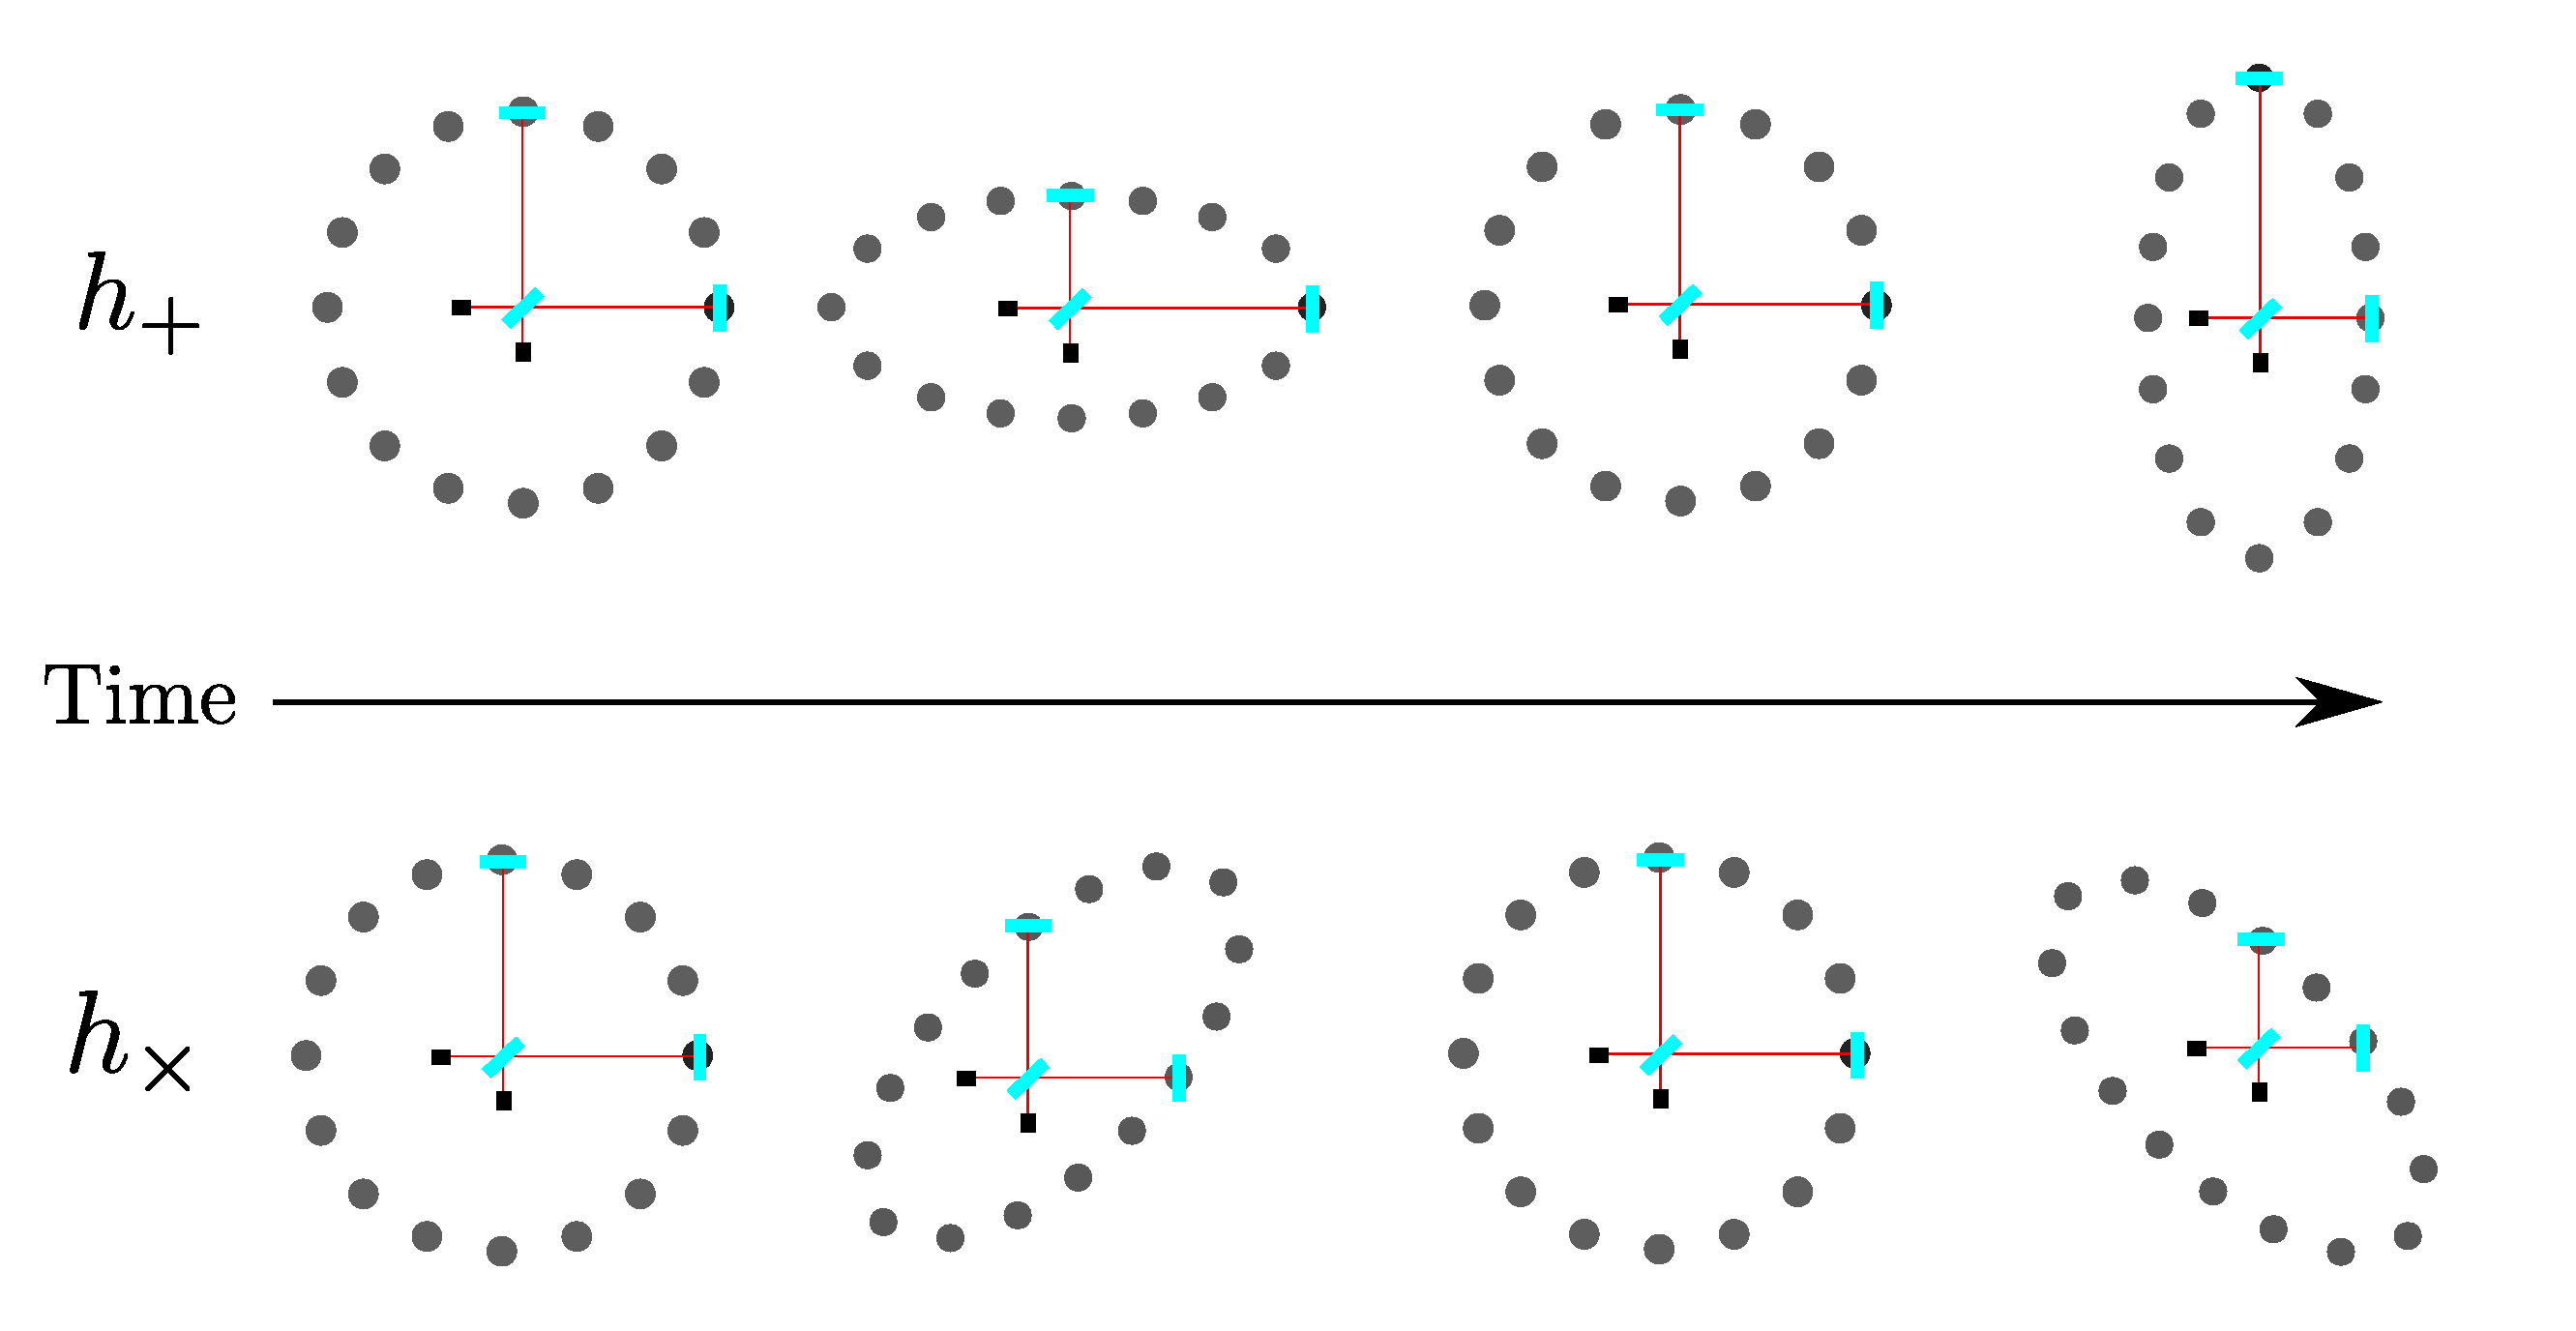
\includegraphics[width=\textwidth]{C1_Introduction/polarisation_ring.pdf}
    \caption{Shows how the plus and cross polarisation's affect a ring of test particles. This assumes the wave is travelling out of the page and the effects have been greatly exaggerated.}
    \label{gw:polarisations}
\end{figure}



\subsubsection{Generating gravitational waves}

To generate gravitational waves we go back to Eq.~\ref{intro:lineinstein} where we include the matter term on the right hand side.
Following the derivation in \citep{Flanagan2005TheTheory}, one can find that the gravitational wave amplitude is related to the second moment of the mass distribution.
The second moment of the mass distribution $I_{\mu\nu}$is defined as,
\begin{equation}
    I_{\mu \nu}(t) = \int \rho(t,{\bf x}) x^\mu x^\nu d^3x,
\end{equation}
where $\rho$ is the mass density, and $x_i$ and $x_j$ are the coordinates \citep{Flanagan2005TheTheory}. 
This is the quadrupole moment tensor without the trace subtracted.
The gravitational wave amplitude is then defined as,
\begin{equation}
\label{intro:gwamp}
    h_{\mu \nu} = \frac{2}{r}  \frac{d^2 I_{\mu \nu}(t-r)}{dt^2}.
\end{equation}
This has a slight modification in the TT gauge, see \citep{Flanagan2005TheTheory}, however, has the same relationship between the mass quarupole and the \ac{GW} amplitude.
This shows that for a \ac{GW} to be generated, the second derivative of the mass quadrupole moment is needed.
A mass quadrupole moment only exists when the mass distribution is not spherically symmetric.
Therefore, a mass which is asymmetric and accelerating will produce a \ac{GW}.

Systems which will produce detectable \acp{GW} are generally rapidly rotating high mass systems which have some asymmetry around their rotation axis.
The sources of these \ac{GW} will be described in the next section.



%%%%%%%%%%%%%%
%%%%%%%%%%%%%
\section{\label{sources}Sources and signals}
%%%%%%%%%%%%%%%
%%%%%%%%%%%%%%%

There are many potential sources for \ac{GW}. The expected sources can be split into 3 general categories based on their signal type: Transient, Stochastic and \acp{CW}.
These categories are chosen based on the length of the signal and how well modelled the signal is.
Fig.~\ref{sources:signaltypes} shows an example of each of the signals as what category they are a part of.
%
\begin{figure}[h]
    \centering
    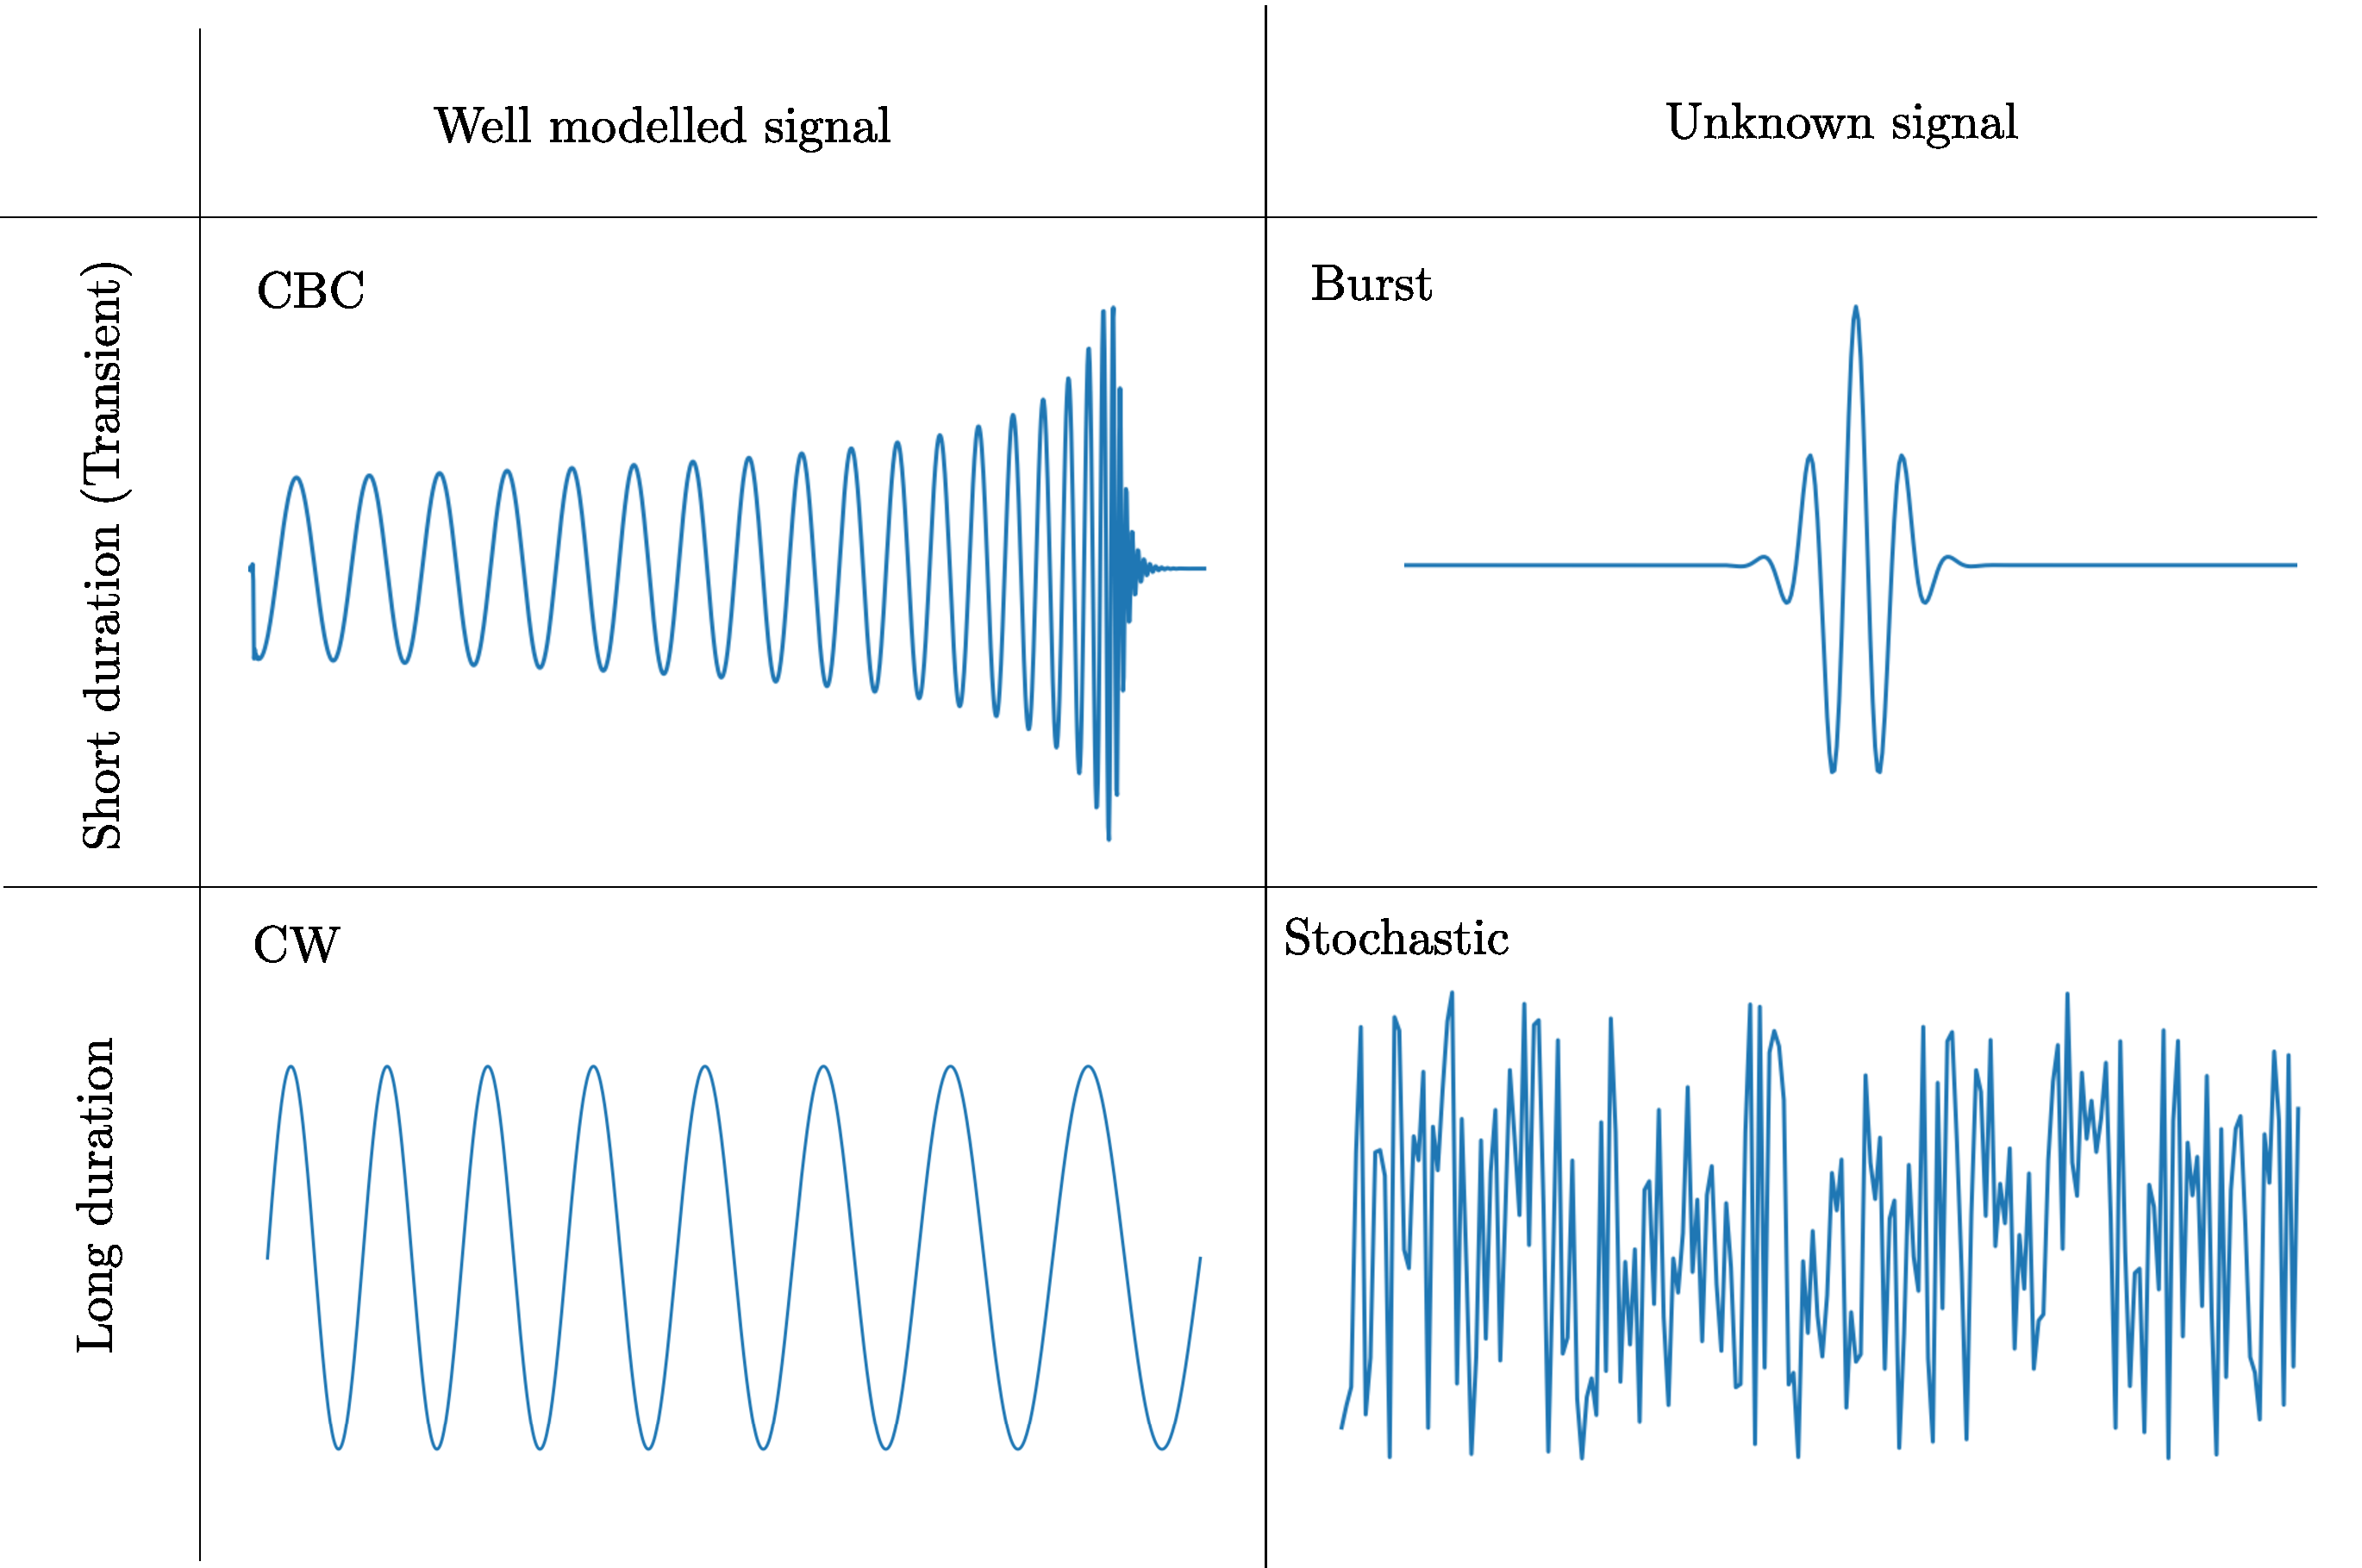
\includegraphics[width=\textwidth]{C1_Introduction/sources_types.pdf}
    \caption{Each \ac{GW} signal type can be categorised based on its signal length and how well the signal is modelled. Transient signals which are short duration, include both well modelled \ac{CBC} signals and unknown Burst signals. Long duration signals include well modelled \ac{CW} signals and unknown Stochastic signals.}
    \label{sources:signaltypes}
\end{figure}
In the sections that follow, I will give an overview of the potential sources of each of these signal categories and their wave-forms.


%%%%%%%%%%%%%%%
\subsection{\label{sources:transient} Transient}
%%%%%%%%%%%%%%%

Transient sources of gravitational waves give short duration signal which is observable from milliseconds to tens of seconds depending on the source. 
Some of these sources will emit signals for a much longer time, however these are at a lower frequency and lower amplitude and not observable by current ground based detectors detectors.
Transient signals can be well modelled as in \acp{CBC} or can have an unknown signal type such as burst signals.

\subsubsection{\label{sources:transient:cbc} Compact Binary Coalescence}

\acp{CBC} originate from two compact objects which are gravitationally bound and eventually collide.
Dependent on the masses of the two objects, the gravitational waves generated by the system can be detected by ground based detector such as LIGO \citep{} and Virgo \citep{}. 
In fact, the only detections to date have been of these signals \citep{}.

The compact objects refered to here refer to either black holes of neutron stars.
There are generally 3 types of \ac{CBC} source: \ac{BBH}, \ac{BNS} and \ac{NSBH}.
The general structure of the waveform follows a `chirp' where the \ac{GW} frequency increases with time until merger. An example of this is shown in Fig.~\ref{sources:signaltypes}.
For higher mass systems such as \ac{BBH} these signals are detectable by ground based detectors for $< 1$s. 
For lower mass systems such as \ac{BNS} they can be detected for longer periods $\mathcal{O}(10)$s. 

The wave-form of a \ac{CBC} signal is generally split into three separate components: the inspiral, the merger and ring-down. 
The inspiral part of the signal is when the objects are orbiting each other. As they lose energy to gravitational waves, the radius of the orbit decreases and therefore the frequency increases.
The merger is the period when the two objects begin to join to become a single object.
The ring-down is the \ac{GW} emitted of the merged object. The joint object can oscillate whilst it settles into its final state. 

In systems which have a neutron star, during the inspiral when the objects are close, the neutron star will begin to deform due to the strong gravity. 
This becomes useful as it will affect the generated waveform and can help determine the \ac{EOS} for the dense matter in a neutron star.
\ac{BNS} systems also offer a way do observe objects in multiple different channels, or what is known as multi-messenger astronomy. 
This is where the object can be viewed in the \ac{EM} spectrum as well as in gravitational waves.
This offers much in the field of astronomy as it can aid in the calculation of the Hubble constant. 

Black hole binaries have various formation channels, i.e. there are different way in which a compact binary system can form. 
These formation channels include: two high mass binary stars which collapse, two separate objects capture each other in their gravitational fields and begin to orbit etc..
However, exactly how common these are or if there are dominant ways in which they form is unknown. 
With many observations of \ac{CBC} it should be possible to discover which of these, if any, is dominant.


%%%%%%%%%%%%%%
\subsubsection{\label{sources:transient:burst}Burst}
%%%%%%%%%%%%%%%%%

Burst sources are also short duration however, are un-modelled or difficult to model.
This mean that the exact wave-form of the signal is unknown.
There are a few possible reasons for the lack in knowledge of the waveform: the physics of the system is too complicated to model in a reasonable amount of time or there is no model of the source.
As there is no model to generate wave-forms, burst searches cannot use matched filtering as in \ac{CBC} searches.
Rather burst searches look for short bursts in power which is coherent between multiple detectors \citep{Cornish2015Bayeswave:Glitches,Klimenko2008ABursts}.

There are a number of systems which could potentially emit a short duration burst signals.
These include core collapse supernovae \citep{Ott2008TheSupernovae}, \acp{GRB} \citep{Aasi2014SearchNetwork}, cosmic strings \citep{Damour2005GravitationalWindows} and other unknown sources.
Detecting \ac{GW} from one of these sources could offer more insight into the processes inside hostile environments.
Burst searches are sensitive to almost any signal which is coherent between detectors. 
This allows them to be used for searches for \ac{CBC} also.



%%%%%%%%%%%%%%%
\subsection{Stochastic}
%%%%%%%%%%%%%%%

The stochastic background has no model for any source, however, is expected to be a persistent source of \ac{GW} in the background of the detector. 
The stochastic background is the incoherent sum of many unresolved \ac{GW} signals.
The source of these signals can be anything from cosmological sources such as cosmic strings to \ac{CBC} signals.
These signals can be thought of as the \ac{GW} analog of the \ac{CMB}.
Where the signal is assumed to be isotropic such that it can be observed at any point on the sky \citep{Christensen2018StochasticBackgrounds}. 
As the stochastic background is essentially just noise, it is not possible to detect with a single detector \citep{Christensen2018StochasticBackgrounds}.
Rather, searches for the stochastic background correlate signals between multiple detectors \citep{Romano2019SearchesBackgrounds,Christensen2018StochasticBackgrounds}. 
When detected, these signals may be able to offer insights into the early universe and its formation.



%%%%%%%%%%%%%%%%%%
\subsection{Continuous waves}
%%%%%%%%%%%%%%%%%%%%

\begin{itemize}
    \item rapidly roating neutron stars main source
    \item long duration continuously emitted
    \item can learn about EOS of dense neutron matter
    \item various emission possiblities
    \begin{itemize}
        \item "mountains" -> magnetic distortions -> crust distortions
        \item fundemental modes inside the neutron star -> fmode -> rmode
        \item precession
    \end{itemize}
    \item have been observed in EM
    \item 
\end{itemize}

Continuous \ac{GW} differ from the above categories as the signals are long duration and are well modelled.
These signals are expected to last for much longer than observing runs of any detector. 

A primary source for continuous signals is expected to be rapidly rotation neutron stars.
Neutron stars are thought to originate when the remnant of a massive star collapses, they are objects with incredibly high density and are highly magnetised.
The strong magnetic fields can funnel material along the field lines towards the magnetic poles and cause the emmission on X-rays or gamma rays.


From electromagnetic observations, the rotation frequency of some pulsars can be observed to decrease with time, this is known as spin-down.
This spin-down means that the pulsar is losing energy somewhere, a fraction of this is thought to be due to gravitational waves. 

To emit gravitational waves the Pulsar has to have some asymmetry in its mass distribution around the rotation axis as spherically symmetric object do not emit gravitational waves.
There are a number of mechanisms which pulsars are thought to be able to emit gravitational waves by. The three leading mechanisms are: non-axisymmetric physical distortions in the star, vibrational modes and free precession \citep{Becker2009}.

%%%%%%
\subsubsection{Triaxial non-axisymmetry}
%%%%%%%%%

Triaxial non-axisymmetry is some deformation of the pulsar which is not symmetric around the rotation axis, this is often described as a `mountain' on its surface.

This assymmetry can be quantified by its ellipticity $\epsilon$,
\begin{equation}
\label{ellipticity}
\epsilon = \frac{I_{xx}-I_{yy}}{I_{zz}},
\end{equation}
where $I_{zz},I_{xx},I_{yy}$ are the principal moment of interia, where $I_{zz}$ is along the rotation axis. 
The ellipticity of a neutron star is expected to be $ \epsilon<10^{-5}$ \citep{Becker2009}. 
There are a number of theories which describe the origin of this axisymmetry.
If the pulsar is in a binary system and accreting material from its companion star, the material can be funnelled towards the magnetic poles by the magnetic field, thereby causing a hot spot.
This `hot spot' could cause a deformation on the surface of the star which is not axi-symmetric. 
The magnetic stresses from strong magnetic fields within the star, could potentially also cause non axi-symmetric deformations to the star.
Finally the spin down of the pulsar itself could cause stresses in the crust of the star until the point of breaking, its then after this break which could leave a distortion in the crust \citep{Becker2009}.

The gravitational waves are expected to be emitted at a frequency which is twice the rotation frequency of the neutron star.
 
 %%%%%%%%%%%%%%
 \subsubsection{Vibrational modes}
 %%%%%%%%%%%%%%%
There are a number of modes within a star such as fundamental (f-modes) and r-modes. 
Each of these waves are oscillation i the star similar to oscillations in the earth which are used for seismology.
The difference between the different modes are the restoring force bringing the perturbed state back to equilibrium.
the f-modes use gravity as the restoring force where the oscillations happen in the crust of the star.
The more promising of these for gravitational wave emission and detection is the r-mode \citep{Becker2009}.
These are oscillations in the superfluid neutron part of the star,
where the restoring force for the oscillations is the Coriolis effect from the rotation of the star.
These are thought to emit gravitational waves at $4/3$ the frequency of rotation \citep{Becker2009}.

%%%%%%%%%%%%%%%
\subsubsection{Free precession}
%%%%%%%%%%%%%%

Free precession is when the rotation axis is misaligned with the symmetry axis of the star so that the start `wobbles'. 
Free precession is expected to produce gravitational waves at a frequency the same as the rotation frequency and twice the rotation frequency \citep{Becker2009}. 


%%%%%%%%%%%%%%%
%%%%%%%%%%%%%%
%%%%%%%%%%%%%%%
\section{\label{intro:detector}Detectors}
%%%%%%%%%%%%%%%%
%%%%%%%%%%%%%%
%%%%%%%%%%%%%%

The theory mentioned above and the indirect detection of gravitational waves from the Hulse-Taylor binary pulsar system left little doubt as to whether \ac{GW} existed. 
The real challenge was to design an instrument which could directly detect gravitational waves.
There were a number of different methods for the design of the instrument which includes: resonant bar detectors, both ground based and space based interferometers, pulsar timing arrays and Cosmic microwave background detectors. 
Resonant bar detectors were initially designed and built by Joseph Weber \citep{}.
These are large cylinders of metal which should resonate as a gravitational wave passes by. 
These detectors did not make a direct detection therefore, the majority of these are no longer operational excluding some alternate designs such as \joe{put the spherical one etc}\citep{}.
Pulsar timing arrays aimed to use the accurate timing of pulsars to measure distortions in space time as a gravitational wave passed between the detector and the pulsar \citep{}. 
Whilst a detection has not been made with this method, these methods are still in use.
Cosmic microwave background detectors aimed to look for evidence of gravitational waves in the polarisations of the CMB \citep{}. 
Despite the announcement of a detection in ..., these are yet to find any evidence.
The most commonly known design of a \ac{GW} detector is the ground based interferometer, these made the first detection of \ac{GW} in 2015 \citep{}.
These are the focus of this section as the analysis that will follow uses data from the \ac{LIGO} detectors in the US.

%%%%%%%%
%%%%%%%%%
\subsection{Laser Interferometers}
%%%%%%%%%%
%%%%%%%%%

Laser interferometers use the interference of light to measure a length with high precision.
A simple design is shown in Fig.~\ref{detectors:interferometer}. 
Here it shows how the laser is equally split into two, each of these beams is sent down perpendicular arms of the detector where then enter a Fabry-Perot cavity \citep{}. 
The light then returns to the beam splitter where the two beams are combined and sent to a photo-detector.
At the output, there is an interference pattern between the two beams.
If the length of one of the arms is changed then the interference pattern will change as the phase of one beam changes with respect to the other.
The Fabry-perot cavity increases the amount of time light stays within the arms and therefore increases the detectors effective arm length. This helps to increase the sensitivity of the detector.
\begin{figure}[h]
    \centering
    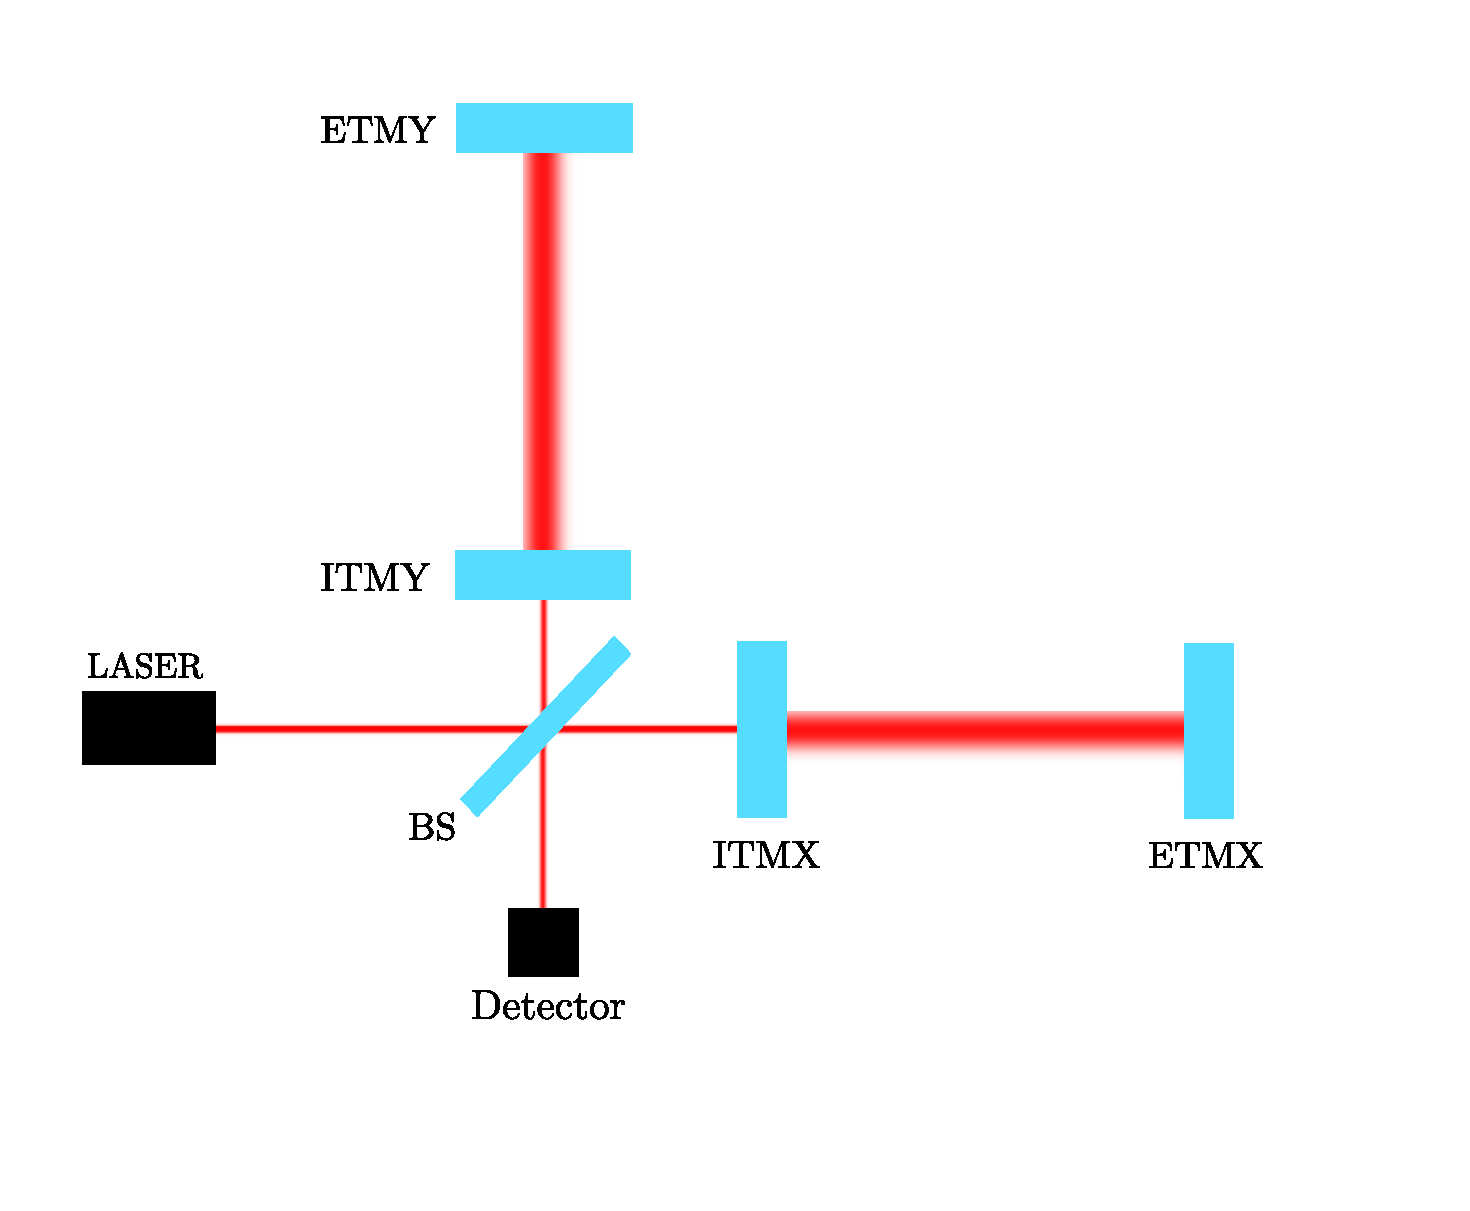
\includegraphics[width=\textwidth]{C1_Introduction/interferometer.pdf}
    \caption{This figure shows a basic interferometer.ETMY and ETMX refer to the external test masses, which are just mirrors at the end of the interferometer arms. ITMY and ITMX refer to the internal test masses, these create a cavity in the interferometers arms which can build up laser power. BS is the beam splitter which splits the Laser beam equally to each arm, this them recombines the beams back to the detector.}
    \label{detectors:interferometer}
\end{figure}

This can be used in gravitational wave detection as the mirrors at the end of each arm of the interfereometer can be treated as `free' test masses.
Fig.~\ref{detectors:interferometer} shows the effect of a \ac{GW} in free test masses.
In the interferometer, this affect essentially changes the relative lengths of the two arms.
The change in the interference pattern with time is then related to the \ac{GW}.
Actual ground based \ac{GW} detectors such as \ac{LIGO} \citep{} and Virgo \citep{} are much more complicated than described above.
They use many techniques to reduce affects on the detector which are not astrophysical.
Some of these effects are listed in Sec.~\ref{intro:detector:noise}


%%%%%%%%%%%
%%%%%%%%%%
\subsubsection{Detector response}
%%%%%%%%%%
%%%%%%%%%

An important factor to know when using detector data to search for astrophysical signals is the detectors response.
This measures how sensitive the detector is to different locations on the sky.
An example of the antenna response for \ac{LIGO} is in Fig.~\ref{detectors:response}.
This is clear when thinking about how a gravitational wave affects the test masses. 
As the affect is transverse to the propagation of the wave, when the detector is face on to the source, there will be a maximum change in the arm lengths.

\begin{figure}
    \centering
    \includegraphics[width=\textwidth]{}
    \caption{This figure shows the antenna response of one of the \ac{LIGO} detectors to sky position.}
    \label{detectors:response}
\end{figure}

%%%%%%%%%%%
%%%%%%%%%%
\subsubsection{\label{intro:detector:noise}Noise sources}
%%%%%%%%%%
%%%%%%%%%%
\begin{enumerate}
    \item Laser interferometers
    \item located US (LIGOs) Virgo
    \item detect the tidal deformations 
    \item mention instrumental lines for later section
    \item sensitivity curves
    \item future detectors
    \item antenna response
    \item 
\end{enumerate}

%%%%%%%%%%%%%
%%%%%%%%%%%%%%%
%%%%%%%%%%%%%%%%
\section{\label{intro:prob}Probability and Bayes Theorem}
%%%%%%%%%%%%%%%
%%%%%%%%%%%%%%%%
%%%%%%%%%%%%%%%%%

A key part in data analysis is understanding probability and statistics. 
This involves using basic probability along with the two general approaches to statistics: Bayesian and frequentist. 

%%%%%%%%%%%%%
%%%%%%%%%%%%%
\subsection{\label{intro:prob:basic}Basic probability}
%%%%%%%%%%%%%%
%%%%%%%%%%%%%%

We can define the probability of some event $A$ as $p(A)$ where probabilities follow $0 \leq p(A) \leq 1$ and some other event $B$ which has a probability $p(B)$ and follows $0 \leq p(B) \leq 1$.

\begin{description}
\item [Union]
A union is the probability of either and event $A$ happening or event $B$ happening, this is written as, $p(A \cup B)$.

\item [Intersection]
An intersection is then the probability of both and event $A$ and an event $B$ happens, this is written as $p(A \cap B)$.

\item [Independent and dependent Events]
If the events $A$ and $B$ are independent, i.e. the event $A$ does not affect the outcome of event $B$, then,
\begin{equation}
p(A \cap B) = p(A)p(B).
\end{equation}
However, if the event $A$ effects event $B$ then the joint probability of both events is,
\begin{equation}
\label{dependentevent}
p(A \cap B) = p(A)p(B \mid A) = p(B)p(A \mid B),
\end{equation}
where $p(B \mid A)$ means the probability of event $B$ happening given that event $A$ has happened.

\item [Conditional probability]
Conditional probability arises from situations where the outcome of one event will affect the outcome of future events.
The definition of this arises from the the dependent events defined above in Eq.~\ref{dependentevent},
\begin{equation}
p(A \mid B) = \frac{p(A \cap B)}{p(B)}.
\end{equation}

\item [Bayes Theorem]
Bayes theorem can then be defined using conditional probabilities. i.e we can use
\begin{equation}
p(A \mid B) = \frac{p(A \cap B)}{p(B)} \quad \rm{and} \quad p(B \mid A) = \frac{p(A \cap B)}{p(A)}
\end{equation}
such that then,
\begin{equation}
p(B)p(A \mid B) = p(A)p(B \mid A)
\end{equation}
and this is rearranged to Bayes theorem,
\begin{equation}
p(A \mid B) = \frac{p(A)p(B \mid A)}{p(B)}
\end{equation}

\end{description}

%%%%%%%%%%%%%%%%%
%%%%%%%%%%%%%%%%%%
\subsection{\label{intro:prob:bayes}Bayesian Inference}
%%%%%%%%%%%%%%%%%%%
%%%%%%%%%%%%%%%

We can take Bayes theorem from Sec.~\ref{intro:prob:basic} and apply it to a problem which involves infering some parameters from some model. Here we can relabel the events $A$ and $B$ with the data ${\bm d}$ and the parameters ${\bm \theta}$ of some model $I$.

\begin{equation}
p({\bm \theta} \mid {\bm d}, I) = \frac{p({\bm \theta}, I)p({\bm d} \mid {\bm \theta}, I)}{p(I)}
\end{equation}
where $p({\bm \theta} \mid {\bm d})$ is the posterior distribution, $p({\bm \theta})$ is the prior distribution,  $p({\bm d} \mid {\bm \theta})$ is the likelihood and $p({\bm d})$ is the evidence.

\begin{description}
\item [Posterior]
The posterior distribution describes the probability of getting certain values of parameters within a model given some data. 
\item [Prior]
The Prior is the element which can be left open to the users interpretation. This describes what you know about the model or the parameters of the model before you have seen any data. 
\item [Likelihood]
The likelihood contains information about how well the data matches the model with particular parameters. 
\item [Evidence]
The evidence is the probability of the data itself, i.e. it explains how likely this data is given and parameters within this model. 
\end{description}

\subsection{MCMC methods}

\subsection{Nested sampling}

